\section{12.7 Metoda Gaussa-Seidla (G-S i S-R -successive relaxation)}

\begin{frame}{Metoda Gaussa-Seidla (G-S i S-R -successive relaxation)}
  $$A=\underbrace{(L+D)}_{B}+U$$
  $$(D+L)x^{(t+1)}=-Ux^t+b$$
  $$\boxed{Dx^{(t+1)}=-Lx^{(t+1)}-Ux^{(t)}+b}$$
  \ \\
  Pamiętamy, że:
  $$x^{(t+1)} = M x^{(t)} + W, M=I-B^{-1}A, W = B^{-1}b$$
  $$M=I-B^{-1}A=I-B^{-1}(B+U)=-B^{-1}U $$
\end{frame}

\begin{frame}{}
  Wzór roboczy:
  $$x^{(t+1)}_i=\frac{1}{a_{ii}}[b_i-\underbrace{\sum^{i-1}_{j=1} a_{ij}x^{(t+1)}_j}_{(\star)}-\underbrace{\sum^{n}_{j=i+1} a_{ij}x^{(t)}_{j}}_{(\star\star)}]$$
   ($\star$) - otrzymujemy z rozwiązania w  bieżącej (t + 1) iteracji, ($\star\star)$ - z poprzedniej iteracji (t).
   \scriptsize{
		    $$
   \varphi^{(t+1)}(x_i,y_j)=
	 \frac{\rho_{i,j}\cdot h^2 +\varphi^{(t+1)}(x_{i},y_{j-1})  + \varphi^{(t+1)}(x_{i-1}, y_j)
	  +\varphi^{(t)}(x_{i+1},y_{j})
	 +\varphi^{(t)}(x_{i},y_{j+1})}{4} 
	 $$
	 }
   \begin{figure}
       \centering
       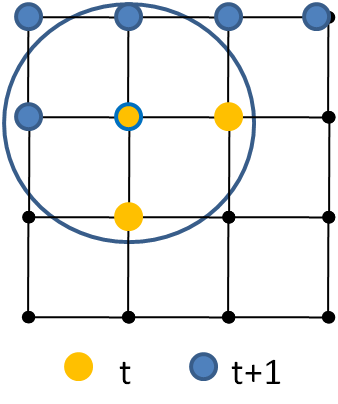
\includegraphics[width=0.25\textwidth]{img/12/gaussseidel.png}
   \end{figure} 
\end{frame}

\begin{frame}{}
  \begin{block}{Charakterystyka metody G-S}
    \begin{itemize}
      \item elementy diagonali powinny być $\neq$ 0 $\rightarrow$ przestawianie
      \item wystarczy pamiętać aktualne przybliżenie $x^{(t+1)}$
      \item zbieżna dla A:
      \begin{itemize}
        \item[*] silnie diagonalnie dominujących wierszowo, kolumnowo,
        \item[*] symetrycznych,
        \item[*] dodatnio określonych $(x^{T}Ax>O\wedge x\neq 0)$.
      \end{itemize}
    \end{itemize}
  \end{block}
\end{frame}
\begin{frame}{}
\begin{block}{Dla modelowego zadania -- met. GS:}
  $$
  \rho(M_{GS})=\rho^2(M_J)
 $$

 $$\lambda_{GS}&=cos^2(\frac{\pi}{N})\approx 1-(\frac{\pi^2}{N^2}) 
   $$
   Metoda GS wymaga dwa razy mniej iteracji niż Jacobiego:
   $$
   R_{GS}=-log_{10}(cos^2(\frac{\pi}{N}))=2R_{J}$$
  $$
  R_{GS}\approx -log_{10}(1-\frac{\pi^2}{N^2})\approx0.4343 \frac{\pi^2}{N^2}
   $$
   \end{block}
          %t^* &= %\frac{ln10}{\pi^2}(pn^2%)...
  
\end{frame}

